\begin{figure}[H]
\centering
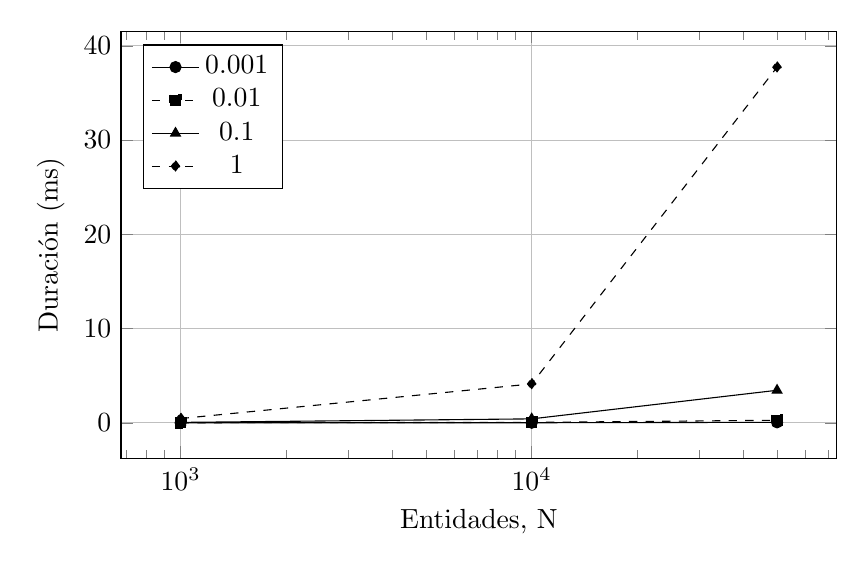
\begin{tikzpicture}
\begin{axis}[width=.88\textwidth,height=7cm,grid=major,legend pos=north west,
xlabel={Entidades, N},ylabel={Duración (ms)},xmode=log,log basis x=10]
\addplot[black,mark=*,solid] coordinates {(1000,0.009667) (10000,0.01) (50000,0.053333)};
\addlegendentry{0.001}
\addplot[black,mark=square*,dashed] coordinates {(1000,0.009166) (10000,0.047084) (50000,0.272458)};
\addlegendentry{0.01}
\addplot[black,mark=triangle*,solid] coordinates {(1000,0.045125) (10000,0.421041) (50000,3.453542)};
\addlegendentry{0.1}
\addplot[black,mark=diamond*,dashed] coordinates {(1000,0.453708) (10000,4.128375) (50000,37.729458)};
\addlegendentry{1}
\end{axis}
\end{tikzpicture}
\caption{Tiempo de reconstrucción incremental por fracción modificada (perfil R).}
\end{figure}